\documentclass[11pt]{article}

\usepackage[margin=1in]{geometry}
\usepackage{fancyhdr}
\usepackage{graphicx}
\pagestyle{fancy}
\usepackage{amsmath}
\usepackage{amssymb}
\usepackage[table]{xcolor}
\usepackage{booktabs}

\lhead{Homework 1}
\chead{Matthew Dees (30281707)}
\rhead{October 9, 2018}


\begin{document}

\begin{enumerate}
\item
\begin{enumerate}
\item The implementation for the 1D optimizer can be found in the {\bf optimizer\_1d.py} file provided in the submission. Within this file the \texttt{optimizer1D(func, initial\_point, initial\_step\_size)} function obeys the prototype mentioned in the assignment and optimizes a function \texttt{func} with starting point \texttt{initial\_start\_point} and step size \texttt{initial\_step\_size}. I used the {\bf golden section} algorithm described in both the book and in class.
\item The two functions I chose to optimize using the 1D unconstrained optimizer developed in part (a) where the following:
\[f(x) = (x - 2)^2 \]
\[f(x) = |x - 5|\]
The stopping criteria used for the algorithm was the following formula from the book:

$$  |x_{1} - x_{3}| \le \epsilon_{R}|x_{2}| + \epsilon_{abs} $$
\centering
OR
$$ |\bar{f} - \bar{f}_{old} | \le \epsilon_{R} |f_{2}| + \epsilon_{abs} $$
\flushleft
Where $\bar{f}$ is the output of the descent function, $\epsilon_{R}$ is the relative machine error ($\sqrt{\epsilon_{m}}$), and $\epsilon_{abs}$ is the absolute error. I used $1.11 \times 10^{-16}$ for the machine error and $1.11 \times 10^{-14}$ for the absolute error.
The following statistics were gathered from 1000 runs using a random \texttt{inital\_point} drawn from the range (-10000, 10000) using the Python \texttt{random.randint()} function. The \texttt{inital\_point} variable was held fixed at 1. The \texttt{random.randint()} function pulled numbers from an approximately uniform distribution over 1000 runs as shown below: \\
\begin{figure}[h]

	\centering
	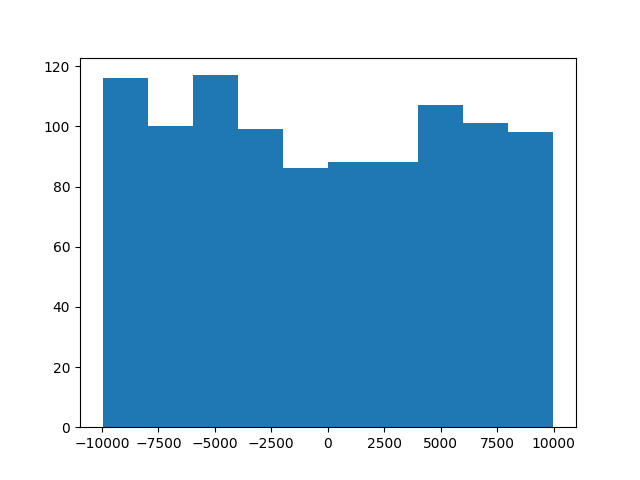
\includegraphics[width=10cm]{report_images/start_point}
	\label{fig:rand_distribution}
	
\end{figure}

All statistics calculations can be found in the {\bf stats\_generator.py} file. The relative distance was calculated using the following formula:

\[\frac{100 \times |x^{*}_{code} - x^{*}_{actual}|}{ {| x^{*}_{actual}|}}\]

 

The statistics below were gathered from the 1,000 runs in the format ${mean} \pm {std. dev.}$. The mean was calculated using:

$$\frac{1}{n} \sum_{i=1}^{n} x_{i}$$
\\
The standard deviation was calculated with the Bessel correction using the formula:

$$\sqrt{ \frac{1}{n - 1} \sum_{i = 1}^{n} (x_{i} - \bar{x})^2}$$

The table statistics were pulled from the output of my program: 
\vspace{5mm}

\begin{tabular}{*4l}    \toprule


	Function    & Num. func. evals  & Run time (ms)  & Relative distance (\%) \\\toprule
	$f(x) = (x - 2)^2$& $57.6 \pm 2.35$ & $8.91 \times 10^{-2} \pm 3.19 \times 10^{-3}$ & $2.85 \times 10^{-10} \pm 1.87 \times 10^{-10}$\\
	$f(x) = |x - 5|$ & $70.4 \pm 3.99$ & $1.10 \times 10^{-1} \pm 5.84 \times 10^{-3}$  & $1.14 \times 10^{-10} \pm 7.49 \times 10^{-11}$\\\\

\end{tabular}

\vspace{5mm}

The following boxplots where created using {\bf graphic\_generator.py} module included in the submission for the same run:

\[f(x) = (x - 2)^2 \]

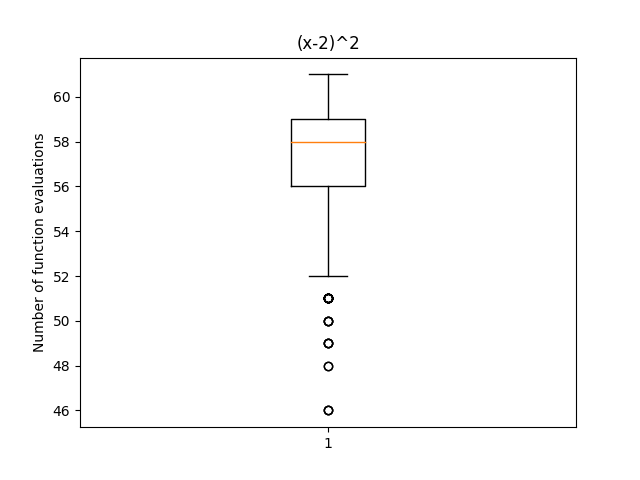
\includegraphics[width=6cm]{report_images/1d_func_1/Number_of_function_evaluations.png}
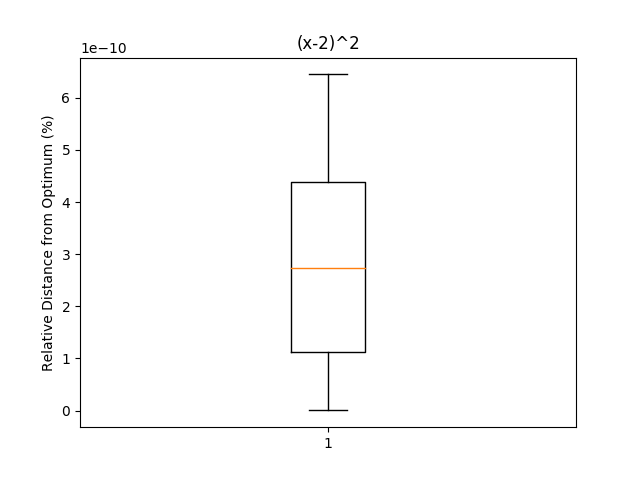
\includegraphics[width=6cm]{report_images/1d_func_1/Relative_Distance_from_Optimum.png}
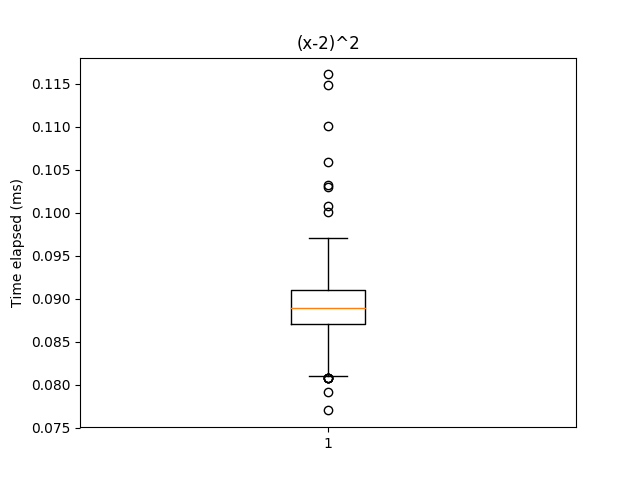
\includegraphics[width=6cm]{report_images/1d_func_1/Time_elapsed.png}

\vspace{50mm}
\[f(x) = |x - 5|\]

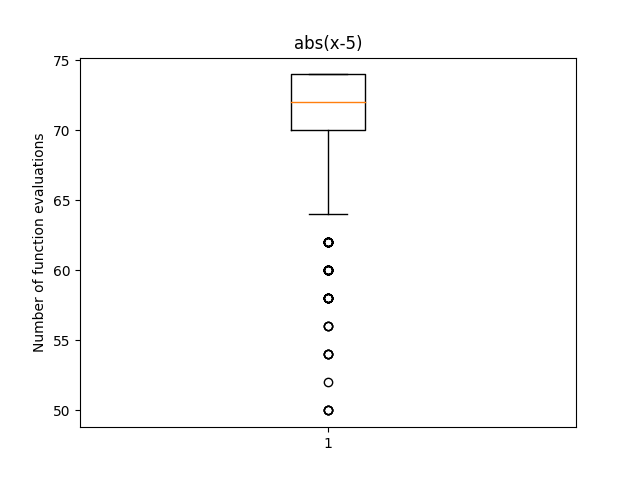
\includegraphics[width=6cm]{report_images/1d_func_2/Number_of_function_evaluations.png}
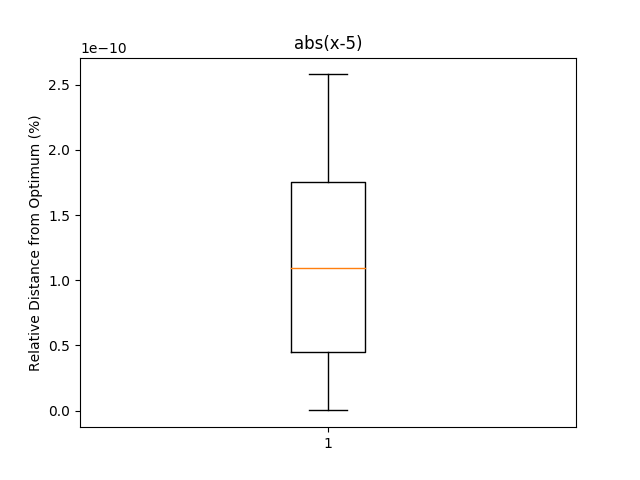
\includegraphics[width=6cm]{report_images/1d_func_2/Relative_Distance_from_Optimum.png}
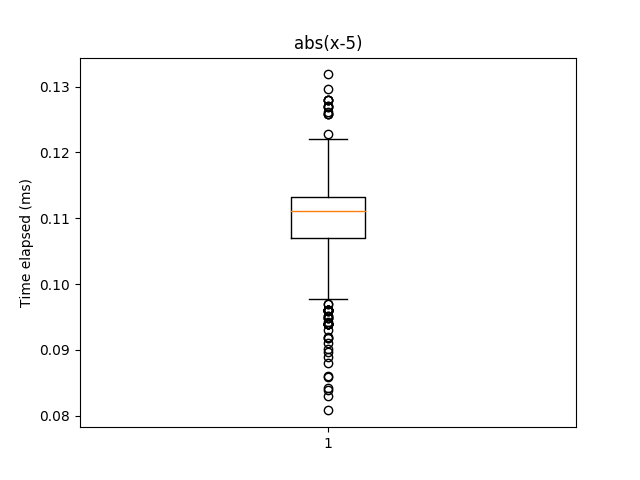
\includegraphics[width=6cm]{report_images/1d_func_2/Time_elapsed.png}

\pagebreak

\end{enumerate}
\item
\begin{enumerate}
	\item My code for the coordinate descent algorithm can be found in the {\bf optimizer\_2d.py} Python file under the \texttt{Optimizer2D} class. There is a global function \texttt{optimizer2D} that can be used to easily evaluate this function using
	the function prototype suggested in the homework assignment.
	\item Most of the statistics formulas used in this part are the same as part (a) in problem 1 above. Some slight modifications needed to be made to support 2 dimensions. The stopping criteria was changed to check the input in all dimensions. If all of the input dimensions satisfied the stopping criteria OR the output criteria (same as output portion of stopping criteria in problem 1) then the 2D algorithm was stopped. This code can be found in the \texttt{should\_stop} function in the \texttt{Optimizer2D} class. 
	The relative distance formula also slightly changed to below formula in order to support multiple dimensions. This code can be found in {\bf stats\_generator.py}.
	$$ 100 \times \frac{||\vec{x}_{code} - \vec{x}_{actual} ||}{||\vec{x}_{actual}||}$$
	
	The following statistics were gathered from running my 2D optimizer with testing infrastructure used in problem 1:
	
	The table statistics were pulled from the output of my program: 
	
	Function 1: $f(x) = 5(x-2.5)^2 - 6(x-2.5)(y-20.5) + 5(y-20.5)^2 $
	
	Function 2: $f(x) = |x - 1| + |y + 5|$
	\vspace{5mm}
	
	\begin{tabular}{*4l}    \toprule
		
		
		Function    & Num. func. evals  & Run time (ms)  & Relative distance (\%) \\\toprule
		 1& $1673 \pm 83.91 $ & $3.9527 \pm 2.213 \times 10^{-1}$ & $5.334 \times 10^{-09} \pm 5.089 \times 10^{-09}$\\
		 2 & $260.3 \pm 4.541$ & $5.400 \times 10^{-1} \pm 1.036 \times 10^{-1}$  & $3.779 \times 10^{-12} \pm 1.719 \times 10^{-12}$\\\\
		
	\end{tabular}
	
	\vspace{5mm}
	
	The following boxplots were retrieved from the graphics generator module included in my submission.
	
	$$f(x) = 5(x-2.5)^2 - 6(x-2.5)(y-20.5) + 5(y-20.5)^2 $$
	
	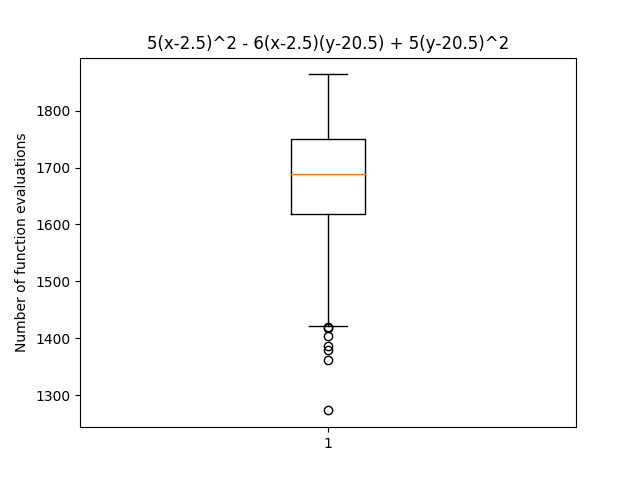
\includegraphics[width=6cm]{report_images/2d_func_1/Number_of_function_evaluations.png}
	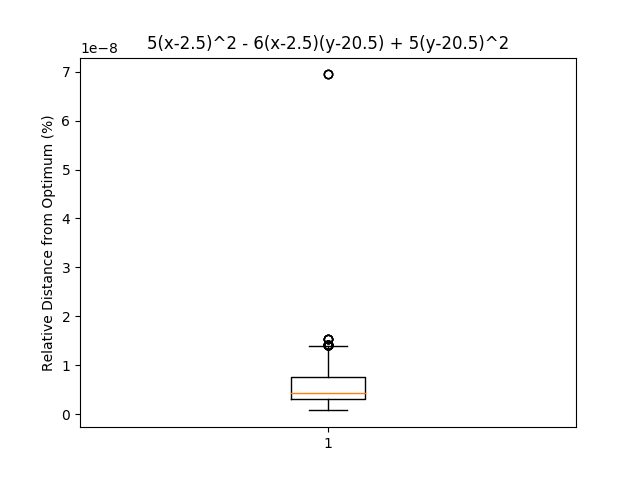
\includegraphics[width=6cm]{report_images/2d_func_1/Relative_Distance_from_Optimum.png}
	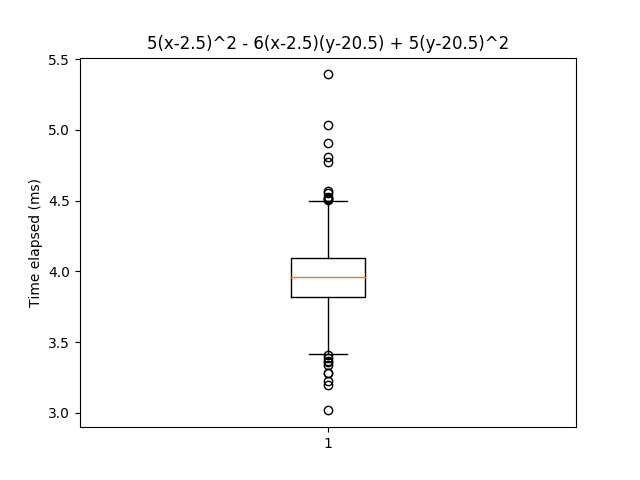
\includegraphics[width=6cm]{report_images/2d_func_1/Time_elapsed.png}
	
	\vspace{50mm}
	$$f(x) = |x - 1| + |y + 5|$$
	
	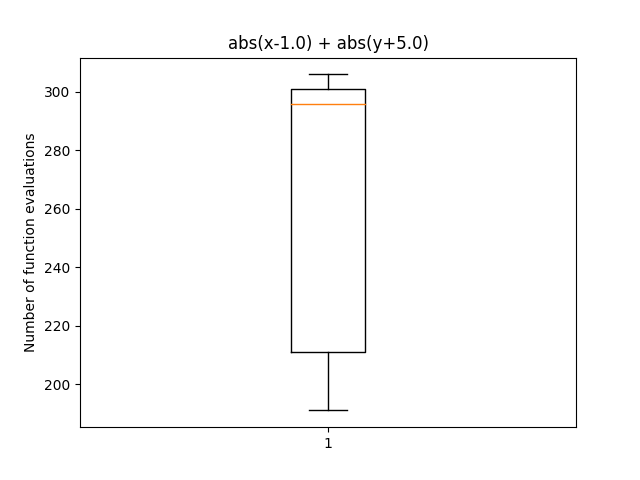
\includegraphics[width=6cm]{report_images/2d_func_2/Number_of_function_evaluations.png}
	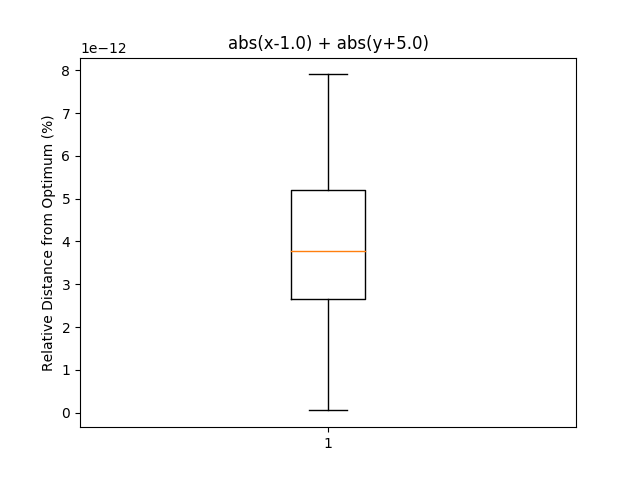
\includegraphics[width=6cm]{report_images/2d_func_2/Relative_Distance_from_Optimum.png}
	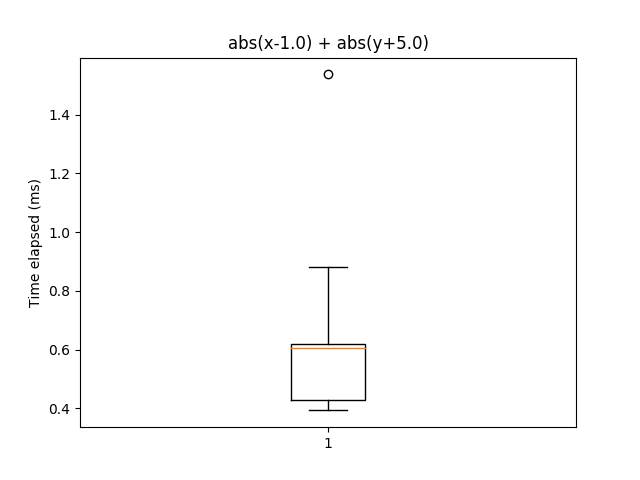
\includegraphics[width=6cm]{report_images/2d_func_2/Time_elapsed.png}
\end{enumerate}



\end{enumerate}
\end{document}